\documentclass[a4paper,12pt]{article}
\special{papersize=210mm,297mm}	% force the paper size to A4
\usepackage[utf8]{inputenc}
\usepackage[english]{babel}
\usepackage{fullpage} % writes text on a fullpage
\usepackage{graphicx} % controls \graphicspath
\usepackage{float} % offers more possibilities to float figures
\usepackage{hyperref} % href command
\usepackage{indentfirst} %with this package is possible to indent the first paragraph of a section
\usepackage{color} %offers the \definecolor command
\usepackage[table]{xcolor}%http://ctan.org/pkg/xcolor
\usepackage{multirow} %allows multirow use in tables
\usepackage{listingsutf8} %used to list code
%\usepackage{epstopdf} %allows the usage of eps in LaTeX

\newcommand{\version}{v14.9.13}
\title{{\LaTeX} tips \& tricks}
\date{September 2014}

\newcommand{\auth}{Andr{{\'e}} Martins}
\newcommand{\authmail}{\small \href{mailto:aanm90@gmail.com}{aanm90@gmail.com}}

\newcommand{\doctitle}{{\LaTeX} tips \& tricks}
\newcommand{\firsttitle}{{\Large \bf{\doctitle}}}

\graphicspath{{images/}}

\definecolor{lgray}{RGB}{230, 230, 230}
\definecolor{dkgreen}{RGB}{0, 230, 0}
\definecolor{ITBlue}{rgb}{0.00,0.32,0.53}
\definecolor{ITRed}{rgb}{0.83,0.05,0.27}

\hypersetup{
    pdfinfo={
        Title={\doctitle},
        Subject={\doctitle},
        Author={\auth},
        Unicode=true
    }
}

\lstset{backgroundcolor=\color{lgray},
    language=[LaTeX]TeX,
    basicstyle=\footnotesize\ttfamily,
    keywordstyle=\bfseries\color{blue},
    commentstyle=\color{dkgreen},
    stringstyle=\ttfamily\color{red},
    firstnumber=1,
    stepnumber=5,
    numbersep=10pt,
    numberstyle=\tiny,
    extendedchars=true,
    breaklines=true,
    tabsize=4,
    showspaces=false,
    showstringspaces=false,
    frame=tb,
    captionpos=b
   % for more info see: http://en.wikibooks.org/wiki/LaTeX/Source_Code_Listings
}

\newcommand\mr[1]{\multirow{2}{*}{#1}}
\newcommand{\superword}{\textit{Supercalifragilisticexpialidocious}}

\begin{document}

\begin{center}
	{\firsttitle} {\version} \\
	{\auth} \\
	{\authmail} \\
\end{center}

\begin{abstract}
This document provides some tips and tricks for your {\LaTeX} documents. If you have any questions you \textbf{must} use \href{www.google.com}{Google}. I will not teach you how to use or create {\LaTeX} documents, this is a tips \& tricks document not a how to use or create {\LaTeX} documents document. This document's .tex is also provided. I am not responsible for any network failure or computer damage that might occur while consulting this document.
\end{abstract}


\tableofcontents

\listoffigures

\section{Figures}

You can refer figures by using \verb|\ref{}|. For example, ``in Figure~\ref{fig:IMGsmall}'' is written as \verb+in Figure~\ref{fig:IMGsmall}+. The use of \verb|~| between \verb|Figure| and \verb|\ref{fig:IMGsmall}| prevents those two words to ``split'' on a line break. Thus, without \verb|~| you will have Figure \ref{fig:IMGsmall}.

\begin{figure}[H]
\centering
\fbox{ %<--- creates a square line around the figure
	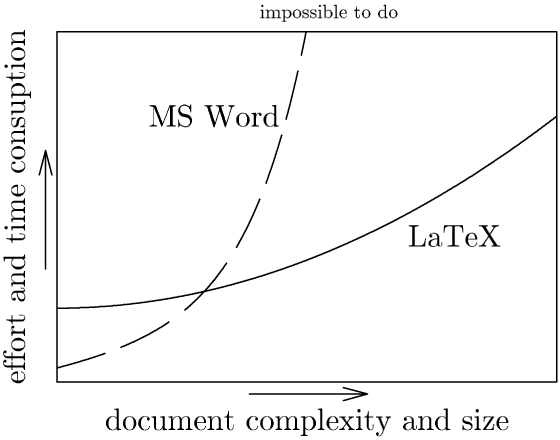
\includegraphics[width=.15\textwidth]{IMG}
}
\caption[A very small image and this text will appear in list of figures.]{A very small image and this text will appear on figure's caption, not in List of Figures.}
\label{fig:IMGsmall}
\end{figure}

\lstinputlisting[firstline=86, lastline=93]{tipsetricks.tex}

Sometimes you need to add a reference where you took that figure from. Figure~\ref{fig:IMGtrimmed}'s source code has an example how it can be done.

%Random comment passing by, there's nothing to see here.

\begin{figure}[H]
\centering
\fbox{ %<--- creates a square line around the figure
	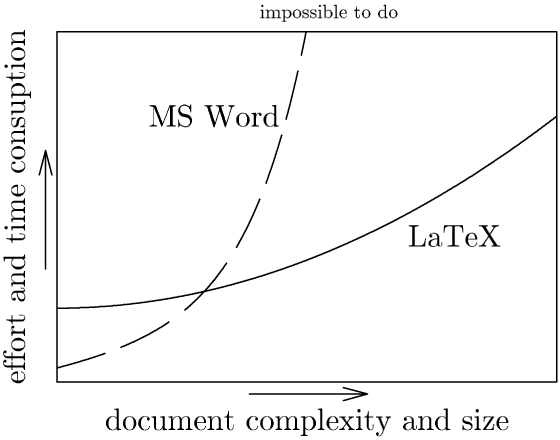
\includegraphics[clip=true,trim=12 25 75 60,width=.8\textwidth]{IMG}
}
\caption[A trimmed image resized to 80\% of {\textbackslash}textwidht and this is useful because the little one doesn't appear here.]{A trimmed image resized to 80\% of {\textbackslash}textwidht~\footnotemark.}
\label{fig:IMGtrimmed}
\end{figure}

\footnotetext{Image available: \url{http://www.pinteric.com/miktex.html}}

\lstinputlisting[firstline=101, lastline=110]{tipsetricks.tex}

You can also use \verb|.pdf| and \verb|.eps| for figures. For \verb|.eps| is necessary to use the package \verb|epstopdf| and the \verb|.eps| files are automatically converted to eps with the name: \verb|EPSFILENAME-eps-converted-to.pdf|

\begin{figure}[H]
\centering
	\includegraphics[page=2,width=.5\textwidth,angle=123,clip=true]{images/tipsetricks}
\caption{A trimmed page of a pdf file resized to half of {\textbackslash}textwidht with a 123 degree angle.}
\label{fig:pdf}
\end{figure}
\lstinputlisting[firstline=116, lastline=121]{tipsetricks.tex}

\section{Tables}
Creating a table is the most annoying thing to do in {\LaTeX}.
Without specifying width for last column we end up with:

\begin{center}
     \begin{tabular}{| l | l | l | l |}
     \hline
     Day & Min Temp & Max Temp & Summary \\ \hline
     Monday & 11C & 22C & A clear day with lots of sunshine.
     However, the strong breeze will bring down the temperatures. \\ \hline
     Tuesday & 9C & 19C & Cloudy with rain, across many northern regions. Clear spells
     across most of Scotland and Northern Ireland,
     but rain reaching the far northwest. \\ \hline
     Wednesday & 10C & 21C & Rain will still linger for the morning.
     Conditions will improve by early afternoon and continue
     throughout the evening. \\
     \hline
     \end{tabular}
\end{center}

With width specified:
 
\begin{center}
     \begin{tabular}{ | l | l | l | p{5cm} |}
     \hline
     Day & Min Temp & Max Temp & Summary \\ \hline
     Monday & 11C & 22C & A clear day with lots of sunshine.  
     However, the strong breeze will bring down the temperatures. \\ \hline
     Tuesday & 9C & 19C & Cloudy with rain, across many northern regions. Clear spells
     across most of Scotland and Northern Ireland,
     but rain reaching the far northwest. \\ \hline
     Wednesday & 10C & 21C & Rain will still linger for the morning.
     Conditions will improve by early afternoon and continue
     throughout the evening. \\
     \hline
     \end{tabular}
\end{center}

\lstinputlisting[firstline=129, lastline=163]{tipsetricks.tex}

For more info see: \url{http://en.wikibooks.org/wiki/LaTeX/Tables}

However, if you use \verb+p{5cm}+ or \verb|p{2cm}| you might end up with a table like the one represented in Table~\ref{table:badtable}.

\begin{table}[tbh!]
  \begin{center}
	\begin{tabular}{|c|p{2cm}|p{5cm}|c|}
		\hline \textbf{Functionalities/Restrictions} & \textbf{This is one of the columns} & \textbf{This is column two with a big word such as {\superword}} & \textbf{{\superword}} \\
		\hline \textbf{\LaTeX} & \mr{Yes} & \mr{No} & \mr{No} \\
		\textbf{is good for you}  & & & \\
		\hline
	\end{tabular} 
 \end{center}
\caption{Reasons to use \LaTeX.}
\label{table:badtable}
\end{table}

\lstinputlisting[firstline=168, lastline=179]{tipsetricks.tex}

This is ugly and you end up with a broken table.
For that reason you can use \newline \verb|\resizebox{h-length}{v-length}{text}| inside table environment and end up with Table~\ref{table:resizedtable}.

\begin{table}[tbh!]
  \begin{center}
    \resizebox{\textwidth}{!}{
		\begin{tabular}{|c|p{2cm}|p{5cm}|c|}
			\hline \textbf{Functionalities/Restrictions} & \textbf{This is one of the columns} & \textbf{This is column two with a big word such as Supercalifragilisticexpialidocious} & \textbf{Supercalifragilisticexpialidocious} \\
			\hline \textbf{\LaTeX} & \mr{Yes} & \multirow{2}{*}{No} & \mr{No} \\
			\textbf{is good for you}  & & & \\
			\hline
		\end{tabular} 
  	} %<---- resizebox ends here!
 \end{center}
\caption{Reasons to use \LaTeX.}
\label{table:resizedtable}
\end{table}

\lstinputlisting[firstline=186, lastline=199]{tipsetricks.tex}

As you might see, there is the command \verb|\mr{}| embracing Yes and No. This command is defined at the beginning of the file, right before \verb|\begin{document}|, as \newline \verb|\newcommand\mr[1]{\multirow{2}{*}{#1}}|. The only reason for using \verb|\mr{}| is to have a more elegant table while reading the .tex file. Multirow allows for a piece of text to be putted  in the middle of $N$ lines \verb|\multirow{N}{*}{Text you want}|.

Is also possible to have colors inside each cell.
\begin{table}[H]
  \begin{center}
  \resizebox{.4\textwidth}{!}{
\begin{tabular}{|c|c|c|c|c|c|c|c|c|c|c|c|c|c|c|c|c|c|c|c|c|c|c|c|c|c|c|c|c|c|c|c|}
\hline
\cellcolor{white} & 	\cellcolor{white} & 	\cellcolor{white} & 	\cellcolor{white} & 	\cellcolor{white} & 	\cellcolor{white} & 	\cellcolor{white} & 	\cellcolor{white} & 	\cellcolor{white} & 	\cellcolor{white} & 	\cellcolor{white} & 	\cellcolor{white} & 	\cellcolor{white} & 	\cellcolor{white} & 	\cellcolor{white} & 	\cellcolor{white} & 	\cellcolor{white} & 	\cellcolor{white} & 	\cellcolor{white} & 	\cellcolor{white} & 	\cellcolor{white} & 	\cellcolor{white} & 	\cellcolor{white} & 	\cellcolor{white} & 	\cellcolor{white} & 	\cellcolor{white} & 	\cellcolor{white} & 	\cellcolor{white} & 	\cellcolor{white} & 	\cellcolor{white} & 	\cellcolor{white} & 	\\	\hline
\cellcolor{white} & 	\cellcolor{white} & 	\cellcolor{white} & 	\cellcolor{white} & 	\cellcolor{white} & 	\cellcolor{white} & 	\cellcolor{white} & 	\cellcolor{white} & 	\cellcolor{white} & 	\cellcolor{white} & 	\cellcolor{white} & 	\cellcolor{white} & 	\cellcolor{white} & 	\cellcolor{white} & 	\cellcolor{white} & 	\cellcolor{white} & 	\cellcolor{white} & 	\cellcolor{white} & 	\cellcolor{white} & 	\cellcolor{white} & 	\cellcolor{white} & 	\cellcolor{ITBlue} & 	\cellcolor{ITBlue} & 	\cellcolor{ITBlue} & 	\cellcolor{white} & 	\cellcolor{white} & 	\cellcolor{white} & 	\cellcolor{white} & 	\cellcolor{white} & 	\cellcolor{white} & 	\cellcolor{white} & 	\\	\hline
\cellcolor{white} & 	\cellcolor{white} & 	\cellcolor{white} & 	\cellcolor{white} & 	\cellcolor{white} & 	\cellcolor{white} & 	\cellcolor{white} & 	\cellcolor{white} & 	\cellcolor{white} & 	\cellcolor{white} & 	\cellcolor{white} & 	\cellcolor{white} & 	\cellcolor{white} & 	\cellcolor{white} & 	\cellcolor{white} & 	\cellcolor{white} & 	\cellcolor{white} & 	\cellcolor{ITBlue} & 	\cellcolor{ITBlue} & 	\cellcolor{ITBlue} & 	\cellcolor{ITBlue} & 	\cellcolor{ITBlue} & 	\cellcolor{ITBlue} & 	\cellcolor{ITBlue} & 	\cellcolor{white} & 	\cellcolor{white} & 	\cellcolor{white} & 	\cellcolor{white} & 	\cellcolor{white} & 	\cellcolor{white} & 	\cellcolor{white} & 	\\	\hline
\cellcolor{white} & 	\cellcolor{white} & 	\cellcolor{white} & 	\cellcolor{white} & 	\cellcolor{white} & 	\cellcolor{white} & 	\cellcolor{white} & 	\cellcolor{white} & 	\cellcolor{white} & 	\cellcolor{white} & 	\cellcolor{white} & 	\cellcolor{white} & 	\cellcolor{white} & 	\cellcolor{white} & 	\cellcolor{ITBlue} & 	\cellcolor{ITBlue} & 	\cellcolor{ITBlue} & 	\cellcolor{ITBlue} & 	\cellcolor{ITBlue} & 	\cellcolor{ITBlue} & 	\cellcolor{ITBlue} & 	\cellcolor{ITBlue} & 	\cellcolor{ITBlue} & 	\cellcolor{ITBlue} & 	\cellcolor{white} & 	\cellcolor{white} & 	\cellcolor{white} & 	\cellcolor{white} & 	\cellcolor{white} & 	\cellcolor{white} & 	\cellcolor{white} & 	\\	\hline
\cellcolor{white} & 	\cellcolor{white} & 	\cellcolor{white} & 	\cellcolor{white} & 	\cellcolor{white} & 	\cellcolor{white} & 	\cellcolor{white} & 	\cellcolor{white} & 	\cellcolor{white} & 	\cellcolor{white} & 	\cellcolor{white} & 	\cellcolor{white} & 	\cellcolor{white} & 	\cellcolor{white} & 	\cellcolor{ITBlue} & 	\cellcolor{ITBlue} & 	\cellcolor{ITBlue} & 	\cellcolor{ITBlue} & 	\cellcolor{ITBlue} & 	\cellcolor{ITBlue} & 	\cellcolor{ITBlue} & 	\cellcolor{ITBlue} & 	\cellcolor{ITBlue} & 	\cellcolor{ITBlue} & 	\cellcolor{white} & 	\cellcolor{white} & 	\cellcolor{white} & 	\cellcolor{white} & 	\cellcolor{white} & 	\cellcolor{white} & 	\cellcolor{white} & 	\\	\hline
\cellcolor{white} & 	\cellcolor{white} & 	\cellcolor{white} & 	\cellcolor{white} & 	\cellcolor{white} & 	\cellcolor{white} & 	\cellcolor{white} & 	\cellcolor{white} & 	\cellcolor{white} & 	\cellcolor{white} & 	\cellcolor{white} & 	\cellcolor{white} & 	\cellcolor{white} & 	\cellcolor{white} & 	\cellcolor{ITBlue} & 	\cellcolor{ITBlue} & 	\cellcolor{ITBlue} & 	\cellcolor{ITBlue} & 	\cellcolor{ITBlue} & 	\cellcolor{ITBlue} & 	\cellcolor{ITBlue} & 	\cellcolor{ITBlue} & 	\cellcolor{ITBlue} & 	\cellcolor{ITBlue} & 	\cellcolor{ITBlue} & 	\cellcolor{ITBlue} & 	\cellcolor{ITBlue} & 	\cellcolor{ITBlue} & 	\cellcolor{ITBlue} & 	\cellcolor{white} & 	\cellcolor{white} & 	\\	\hline
\cellcolor{white} & 	\cellcolor{white} & 	\cellcolor{white} & 	\cellcolor{white} & 	\cellcolor{white} & 	\cellcolor{white} & 	\cellcolor{white} & 	\cellcolor{white} & 	\cellcolor{white} & 	\cellcolor{white} & 	\cellcolor{white} & 	\cellcolor{white} & 	\cellcolor{white} & 	\cellcolor{white} & 	\cellcolor{ITBlue} & 	\cellcolor{ITBlue} & 	\cellcolor{ITBlue} & 	\cellcolor{ITBlue} & 	\cellcolor{ITBlue} & 	\cellcolor{ITBlue} & 	\cellcolor{ITBlue} & 	\cellcolor{ITBlue} & 	\cellcolor{ITBlue} & 	\cellcolor{ITBlue} & 	\cellcolor{ITBlue} & 	\cellcolor{ITBlue} & 	\cellcolor{ITBlue} & 	\cellcolor{ITBlue} & 	\cellcolor{ITBlue} & 	\cellcolor{white} & 	\cellcolor{white} & 	\\	\hline
\cellcolor{white} & 	\cellcolor{white} & 	\cellcolor{white} & 	\cellcolor{white} & 	\cellcolor{white} & 	\cellcolor{white} & 	\cellcolor{white} & 	\cellcolor{white} & 	\cellcolor{white} & 	\cellcolor{white} & 	\cellcolor{white} & 	\cellcolor{white} & 	\cellcolor{white} & 	\cellcolor{white} & 	\cellcolor{ITBlue} & 	\cellcolor{ITBlue} & 	\cellcolor{ITBlue} & 	\cellcolor{ITBlue} & 	\cellcolor{ITBlue} & 	\cellcolor{ITBlue} & 	\cellcolor{ITBlue} & 	\cellcolor{ITBlue} & 	\cellcolor{ITBlue} & 	\cellcolor{ITBlue} & 	\cellcolor{ITBlue} & 	\cellcolor{ITBlue} & 	\cellcolor{ITBlue} & 	\cellcolor{ITBlue} & 	\cellcolor{ITBlue} & 	\cellcolor{white} & 	\cellcolor{white} & 	\\	\hline
\cellcolor{white} & 	\cellcolor{white} & 	\cellcolor{white} & 	\cellcolor{white} & 	\cellcolor{white} & 	\cellcolor{white} & 	\cellcolor{white} & 	\cellcolor{white} & 	\cellcolor{white} & 	\cellcolor{white} & 	\cellcolor{ITRed} & 	\cellcolor{ITRed} & 	\cellcolor{white} & 	\cellcolor{white} & 	\cellcolor{ITBlue} & 	\cellcolor{ITBlue} & 	\cellcolor{ITBlue} & 	\cellcolor{ITBlue} & 	\cellcolor{ITBlue} & 	\cellcolor{ITBlue} & 	\cellcolor{ITBlue} & 	\cellcolor{ITBlue} & 	\cellcolor{ITBlue} & 	\cellcolor{ITBlue} & 	\cellcolor{ITBlue} & 	\cellcolor{ITBlue} & 	\cellcolor{ITBlue} & 	\cellcolor{ITBlue} & 	\cellcolor{ITBlue} & 	\cellcolor{white} & 	\cellcolor{white} & 	\\	\hline
\cellcolor{white} & 	\cellcolor{white} & 	\cellcolor{white} & 	\cellcolor{white} & 	\cellcolor{white} & 	\cellcolor{white} & 	\cellcolor{white} & 	\cellcolor{white} & 	\cellcolor{white} & 	\cellcolor{ITRed} & 	\cellcolor{ITRed} & 	\cellcolor{ITRed} & 	\cellcolor{ITRed} & 	\cellcolor{white} & 	\cellcolor{ITBlue} & 	\cellcolor{ITBlue} & 	\cellcolor{ITBlue} & 	\cellcolor{ITBlue} & 	\cellcolor{ITBlue} & 	\cellcolor{ITBlue} & 	\cellcolor{ITBlue} & 	\cellcolor{ITBlue} & 	\cellcolor{ITBlue} & 	\cellcolor{ITBlue} & 	\cellcolor{ITBlue} & 	\cellcolor{ITBlue} & 	\cellcolor{ITBlue} & 	\cellcolor{ITBlue} & 	\cellcolor{ITBlue} & 	\cellcolor{white} & 	\cellcolor{white} & 	\\	\hline
\cellcolor{white} & 	\cellcolor{white} & 	\cellcolor{white} & 	\cellcolor{white} & 	\cellcolor{white} & 	\cellcolor{white} & 	\cellcolor{white} & 	\cellcolor{white} & 	\cellcolor{ITRed} & 	\cellcolor{ITRed} & 	\cellcolor{ITRed} & 	\cellcolor{ITRed} & 	\cellcolor{ITRed} & 	\cellcolor{white} & 	\cellcolor{ITBlue} & 	\cellcolor{ITBlue} & 	\cellcolor{ITBlue} & 	\cellcolor{ITBlue} & 	\cellcolor{ITBlue} & 	\cellcolor{ITBlue} & 	\cellcolor{ITBlue} & 	\cellcolor{ITBlue} & 	\cellcolor{ITBlue} & 	\cellcolor{ITBlue} & 	\cellcolor{ITBlue} & 	\cellcolor{ITBlue} & 	\cellcolor{ITBlue} & 	\cellcolor{ITBlue} & 	\cellcolor{ITBlue} & 	\cellcolor{white} & 	\cellcolor{white} & 	\\	\hline
\cellcolor{white} & 	\cellcolor{white} & 	\cellcolor{white} & 	\cellcolor{white} & 	\cellcolor{white} & 	\cellcolor{white} & 	\cellcolor{white} & 	\cellcolor{ITRed} & 	\cellcolor{ITRed} & 	\cellcolor{ITRed} & 	\cellcolor{ITRed} & 	\cellcolor{ITRed} & 	\cellcolor{ITRed} & 	\cellcolor{white} & 	\cellcolor{ITBlue} & 	\cellcolor{ITBlue} & 	\cellcolor{ITBlue} & 	\cellcolor{ITBlue} & 	\cellcolor{ITBlue} & 	\cellcolor{ITBlue} & 	\cellcolor{ITBlue} & 	\cellcolor{ITBlue} & 	\cellcolor{ITBlue} & 	\cellcolor{ITBlue} & 	\cellcolor{ITBlue} & 	\cellcolor{ITBlue} & 	\cellcolor{ITBlue} & 	\cellcolor{ITBlue} & 	\cellcolor{ITBlue} & 	\cellcolor{white} & 	\cellcolor{white} & 	\\	\hline
\cellcolor{white} & 	\cellcolor{white} & 	\cellcolor{white} & 	\cellcolor{white} & 	\cellcolor{white} & 	\cellcolor{white} & 	\cellcolor{ITRed} & 	\cellcolor{ITRed} & 	\cellcolor{ITRed} & 	\cellcolor{ITRed} & 	\cellcolor{ITRed} & 	\cellcolor{ITRed} & 	\cellcolor{ITRed} & 	\cellcolor{white} & 	\cellcolor{ITBlue} & 	\cellcolor{ITBlue} & 	\cellcolor{ITBlue} & 	\cellcolor{ITBlue} & 	\cellcolor{ITBlue} & 	\cellcolor{ITBlue} & 	\cellcolor{ITBlue} & 	\cellcolor{ITBlue} & 	\cellcolor{ITBlue} & 	\cellcolor{ITBlue} & 	\cellcolor{ITBlue} & 	\cellcolor{ITBlue} & 	\cellcolor{white} & 	\cellcolor{white} & 	\cellcolor{white} & 	\cellcolor{white} & 	\cellcolor{white} & 	\\	\hline
\cellcolor{white} & 	\cellcolor{white} & 	\cellcolor{white} & 	\cellcolor{white} & 	\cellcolor{white} & 	\cellcolor{ITRed} & 	\cellcolor{ITRed} & 	\cellcolor{ITRed} & 	\cellcolor{ITRed} & 	\cellcolor{ITRed} & 	\cellcolor{ITRed} & 	\cellcolor{ITRed} & 	\cellcolor{white} & 	\cellcolor{white} & 	\cellcolor{ITBlue} & 	\cellcolor{ITBlue} & 	\cellcolor{ITBlue} & 	\cellcolor{ITBlue} & 	\cellcolor{ITBlue} & 	\cellcolor{ITBlue} & 	\cellcolor{ITBlue} & 	\cellcolor{ITBlue} & 	\cellcolor{ITBlue} & 	\cellcolor{ITBlue} & 	\cellcolor{white} & 	\cellcolor{white} & 	\cellcolor{white} & 	\cellcolor{white} & 	\cellcolor{white} & 	\cellcolor{white} & 	\cellcolor{white} & 	\\	\hline
\cellcolor{white} & 	\cellcolor{white} & 	\cellcolor{white} & 	\cellcolor{white} & 	\cellcolor{ITRed} & 	\cellcolor{ITRed} & 	\cellcolor{ITRed} & 	\cellcolor{ITRed} & 	\cellcolor{ITRed} & 	\cellcolor{ITRed} & 	\cellcolor{ITRed} & 	\cellcolor{white} & 	\cellcolor{white} & 	\cellcolor{white} & 	\cellcolor{ITBlue} & 	\cellcolor{ITBlue} & 	\cellcolor{ITBlue} & 	\cellcolor{ITBlue} & 	\cellcolor{ITBlue} & 	\cellcolor{ITBlue} & 	\cellcolor{ITBlue} & 	\cellcolor{ITBlue} & 	\cellcolor{ITBlue} & 	\cellcolor{ITBlue} & 	\cellcolor{white} & 	\cellcolor{white} & 	\cellcolor{white} & 	\cellcolor{white} & 	\cellcolor{white} & 	\cellcolor{white} & 	\cellcolor{white} & 	\\	\hline
\cellcolor{white} & 	\cellcolor{white} & 	\cellcolor{white} & 	\cellcolor{ITRed} & 	\cellcolor{ITRed} & 	\cellcolor{ITRed} & 	\cellcolor{ITRed} & 	\cellcolor{ITRed} & 	\cellcolor{ITRed} & 	\cellcolor{ITRed} & 	\cellcolor{white} & 	\cellcolor{white} & 	\cellcolor{white} & 	\cellcolor{white} & 	\cellcolor{ITBlue} & 	\cellcolor{ITBlue} & 	\cellcolor{ITBlue} & 	\cellcolor{ITBlue} & 	\cellcolor{ITBlue} & 	\cellcolor{ITBlue} & 	\cellcolor{ITBlue} & 	\cellcolor{ITBlue} & 	\cellcolor{ITBlue} & 	\cellcolor{ITBlue} & 	\cellcolor{white} & 	\cellcolor{white} & 	\cellcolor{white} & 	\cellcolor{white} & 	\cellcolor{white} & 	\cellcolor{white} & 	\cellcolor{white} & 	\\	\hline
\cellcolor{white} & 	\cellcolor{white} & 	\cellcolor{white} & 	\cellcolor{white} & 	\cellcolor{ITRed} & 	\cellcolor{ITRed} & 	\cellcolor{ITRed} & 	\cellcolor{ITRed} & 	\cellcolor{white} & 	\cellcolor{white} & 	\cellcolor{white} & 	\cellcolor{white} & 	\cellcolor{ITBlue} & 	\cellcolor{white} & 	\cellcolor{ITBlue} & 	\cellcolor{ITBlue} & 	\cellcolor{ITBlue} & 	\cellcolor{ITBlue} & 	\cellcolor{ITBlue} & 	\cellcolor{ITBlue} & 	\cellcolor{ITBlue} & 	\cellcolor{ITBlue} & 	\cellcolor{ITBlue} & 	\cellcolor{ITBlue} & 	\cellcolor{white} & 	\cellcolor{white} & 	\cellcolor{white} & 	\cellcolor{white} & 	\cellcolor{white} & 	\cellcolor{white} & 	\cellcolor{white} & 	\\	\hline
\cellcolor{white} & 	\cellcolor{white} & 	\cellcolor{white} & 	\cellcolor{white} & 	\cellcolor{white} & 	\cellcolor{white} & 	\cellcolor{white} & 	\cellcolor{white} & 	\cellcolor{white} & 	\cellcolor{ITBlue} & 	\cellcolor{ITBlue} & 	\cellcolor{ITBlue} & 	\cellcolor{ITBlue} & 	\cellcolor{white} & 	\cellcolor{ITBlue} & 	\cellcolor{ITBlue} & 	\cellcolor{ITBlue} & 	\cellcolor{ITBlue} & 	\cellcolor{ITBlue} & 	\cellcolor{ITBlue} & 	\cellcolor{ITBlue} & 	\cellcolor{ITBlue} & 	\cellcolor{ITBlue} & 	\cellcolor{ITBlue} & 	\cellcolor{white} & 	\cellcolor{white} & 	\cellcolor{white} & 	\cellcolor{white} & 	\cellcolor{white} & 	\cellcolor{white} & 	\cellcolor{white} & 	\\	\hline
\cellcolor{white} & 	\cellcolor{white} & 	\cellcolor{white} & 	\cellcolor{white} & 	\cellcolor{white} & 	\cellcolor{white} & 	\cellcolor{ITBlue} & 	\cellcolor{ITBlue} & 	\cellcolor{ITBlue} & 	\cellcolor{ITBlue} & 	\cellcolor{ITBlue} & 	\cellcolor{ITBlue} & 	\cellcolor{ITBlue} & 	\cellcolor{white} & 	\cellcolor{ITBlue} & 	\cellcolor{ITBlue} & 	\cellcolor{ITBlue} & 	\cellcolor{ITBlue} & 	\cellcolor{ITBlue} & 	\cellcolor{ITBlue} & 	\cellcolor{ITBlue} & 	\cellcolor{ITBlue} & 	\cellcolor{ITBlue} & 	\cellcolor{ITBlue} & 	\cellcolor{white} & 	\cellcolor{white} & 	\cellcolor{white} & 	\cellcolor{white} & 	\cellcolor{white} & 	\cellcolor{white} & 	\cellcolor{white} & 	\\	\hline
\cellcolor{white} & 	\cellcolor{white} & 	\cellcolor{white} & 	\cellcolor{ITBlue} & 	\cellcolor{ITBlue} & 	\cellcolor{ITBlue} & 	\cellcolor{ITBlue} & 	\cellcolor{ITBlue} & 	\cellcolor{ITBlue} & 	\cellcolor{ITBlue} & 	\cellcolor{ITBlue} & 	\cellcolor{ITBlue} & 	\cellcolor{ITBlue} & 	\cellcolor{white} & 	\cellcolor{ITBlue} & 	\cellcolor{ITBlue} & 	\cellcolor{ITBlue} & 	\cellcolor{ITBlue} & 	\cellcolor{ITBlue} & 	\cellcolor{ITBlue} & 	\cellcolor{ITBlue} & 	\cellcolor{ITBlue} & 	\cellcolor{ITBlue} & 	\cellcolor{ITBlue} & 	\cellcolor{white} & 	\cellcolor{white} & 	\cellcolor{white} & 	\cellcolor{white} & 	\cellcolor{white} & 	\cellcolor{white} & 	\cellcolor{white} & 	\\	\hline
\cellcolor{white} & 	\cellcolor{white} & 	\cellcolor{white} & 	\cellcolor{ITBlue} & 	\cellcolor{ITBlue} & 	\cellcolor{ITBlue} & 	\cellcolor{ITBlue} & 	\cellcolor{ITBlue} & 	\cellcolor{ITBlue} & 	\cellcolor{ITBlue} & 	\cellcolor{ITBlue} & 	\cellcolor{ITBlue} & 	\cellcolor{ITBlue} & 	\cellcolor{white} & 	\cellcolor{ITBlue} & 	\cellcolor{ITBlue} & 	\cellcolor{ITBlue} & 	\cellcolor{ITBlue} & 	\cellcolor{ITBlue} & 	\cellcolor{ITBlue} & 	\cellcolor{ITBlue} & 	\cellcolor{ITBlue} & 	\cellcolor{ITBlue} & 	\cellcolor{ITBlue} & 	\cellcolor{white} & 	\cellcolor{white} & 	\cellcolor{white} & 	\cellcolor{white} & 	\cellcolor{white} & 	\cellcolor{white} & 	\cellcolor{white} & 	\\	\hline
\cellcolor{white} & 	\cellcolor{white} & 	\cellcolor{white} & 	\cellcolor{ITBlue} & 	\cellcolor{ITBlue} & 	\cellcolor{ITBlue} & 	\cellcolor{ITBlue} & 	\cellcolor{ITBlue} & 	\cellcolor{ITBlue} & 	\cellcolor{ITBlue} & 	\cellcolor{ITBlue} & 	\cellcolor{ITBlue} & 	\cellcolor{ITBlue} & 	\cellcolor{white} & 	\cellcolor{ITBlue} & 	\cellcolor{ITBlue} & 	\cellcolor{ITBlue} & 	\cellcolor{ITBlue} & 	\cellcolor{ITBlue} & 	\cellcolor{ITBlue} & 	\cellcolor{ITBlue} & 	\cellcolor{ITBlue} & 	\cellcolor{ITBlue} & 	\cellcolor{ITBlue} & 	\cellcolor{white} & 	\cellcolor{white} & 	\cellcolor{white} & 	\cellcolor{white} & 	\cellcolor{white} & 	\cellcolor{white} & 	\cellcolor{white} & 	\\	\hline
\cellcolor{white} & 	\cellcolor{white} & 	\cellcolor{white} & 	\cellcolor{ITBlue} & 	\cellcolor{ITBlue} & 	\cellcolor{ITBlue} & 	\cellcolor{ITBlue} & 	\cellcolor{ITBlue} & 	\cellcolor{ITBlue} & 	\cellcolor{ITBlue} & 	\cellcolor{ITBlue} & 	\cellcolor{ITBlue} & 	\cellcolor{ITBlue} & 	\cellcolor{white} & 	\cellcolor{ITBlue} & 	\cellcolor{ITBlue} & 	\cellcolor{ITBlue} & 	\cellcolor{ITBlue} & 	\cellcolor{ITBlue} & 	\cellcolor{ITBlue} & 	\cellcolor{ITBlue} & 	\cellcolor{ITBlue} & 	\cellcolor{ITBlue} & 	\cellcolor{ITBlue} & 	\cellcolor{ITBlue} & 	\cellcolor{ITBlue} & 	\cellcolor{ITBlue} & 	\cellcolor{ITBlue} & 	\cellcolor{ITBlue} & 	\cellcolor{white} & 	\cellcolor{white} & 	\\	\hline
\cellcolor{white} & 	\cellcolor{white} & 	\cellcolor{white} & 	\cellcolor{ITBlue} & 	\cellcolor{ITBlue} & 	\cellcolor{ITBlue} & 	\cellcolor{ITBlue} & 	\cellcolor{ITBlue} & 	\cellcolor{ITBlue} & 	\cellcolor{ITBlue} & 	\cellcolor{ITBlue} & 	\cellcolor{ITBlue} & 	\cellcolor{ITBlue} & 	\cellcolor{white} & 	\cellcolor{ITBlue} & 	\cellcolor{ITBlue} & 	\cellcolor{ITBlue} & 	\cellcolor{ITBlue} & 	\cellcolor{ITBlue} & 	\cellcolor{ITBlue} & 	\cellcolor{ITBlue} & 	\cellcolor{ITBlue} & 	\cellcolor{ITBlue} & 	\cellcolor{ITBlue} & 	\cellcolor{ITBlue} & 	\cellcolor{ITBlue} & 	\cellcolor{ITBlue} & 	\cellcolor{ITBlue} & 	\cellcolor{ITBlue} & 	\cellcolor{white} & 	\cellcolor{white} & 	\\	\hline
\cellcolor{white} & 	\cellcolor{white} & 	\cellcolor{white} & 	\cellcolor{ITBlue} & 	\cellcolor{ITBlue} & 	\cellcolor{ITBlue} & 	\cellcolor{ITBlue} & 	\cellcolor{ITBlue} & 	\cellcolor{ITBlue} & 	\cellcolor{ITBlue} & 	\cellcolor{ITBlue} & 	\cellcolor{ITBlue} & 	\cellcolor{ITBlue} & 	\cellcolor{white} & 	\cellcolor{ITBlue} & 	\cellcolor{ITBlue} & 	\cellcolor{ITBlue} & 	\cellcolor{ITBlue} & 	\cellcolor{ITBlue} & 	\cellcolor{ITBlue} & 	\cellcolor{ITBlue} & 	\cellcolor{ITBlue} & 	\cellcolor{ITBlue} & 	\cellcolor{ITBlue} & 	\cellcolor{ITBlue} & 	\cellcolor{ITBlue} & 	\cellcolor{ITBlue} & 	\cellcolor{ITBlue} & 	\cellcolor{ITBlue} & 	\cellcolor{white} & 	\cellcolor{white} & 	\\	\hline
\cellcolor{white} & 	\cellcolor{white} & 	\cellcolor{white} & 	\cellcolor{ITBlue} & 	\cellcolor{ITBlue} & 	\cellcolor{ITBlue} & 	\cellcolor{ITBlue} & 	\cellcolor{ITBlue} & 	\cellcolor{ITBlue} & 	\cellcolor{ITBlue} & 	\cellcolor{ITBlue} & 	\cellcolor{ITBlue} & 	\cellcolor{ITBlue} & 	\cellcolor{white} & 	\cellcolor{white} & 	\cellcolor{ITBlue} & 	\cellcolor{ITBlue} & 	\cellcolor{ITBlue} & 	\cellcolor{ITBlue} & 	\cellcolor{ITBlue} & 	\cellcolor{ITBlue} & 	\cellcolor{ITBlue} & 	\cellcolor{ITBlue} & 	\cellcolor{ITBlue} & 	\cellcolor{ITBlue} & 	\cellcolor{ITBlue} & 	\cellcolor{ITBlue} & 	\cellcolor{ITBlue} & 	\cellcolor{ITBlue} & 	\cellcolor{white} & 	\cellcolor{white} & 	\\	\hline
\cellcolor{white} & 	\cellcolor{white} & 	\cellcolor{white} & 	\cellcolor{ITBlue} & 	\cellcolor{ITBlue} & 	\cellcolor{ITBlue} & 	\cellcolor{ITBlue} & 	\cellcolor{ITBlue} & 	\cellcolor{ITBlue} & 	\cellcolor{ITBlue} & 	\cellcolor{ITBlue} & 	\cellcolor{ITBlue} & 	\cellcolor{ITBlue} & 	\cellcolor{white} & 	\cellcolor{white} & 	\cellcolor{white} & 	\cellcolor{ITBlue} & 	\cellcolor{ITBlue} & 	\cellcolor{ITBlue} & 	\cellcolor{ITBlue} & 	\cellcolor{ITBlue} & 	\cellcolor{ITBlue} & 	\cellcolor{ITBlue} & 	\cellcolor{ITBlue} & 	\cellcolor{ITBlue} & 	\cellcolor{ITBlue} & 	\cellcolor{ITBlue} & 	\cellcolor{ITBlue} & 	\cellcolor{ITBlue} & 	\cellcolor{white} & 	\cellcolor{white} & 	\\	\hline
\cellcolor{white} & 	\cellcolor{white} & 	\cellcolor{white} & 	\cellcolor{ITBlue} & 	\cellcolor{ITBlue} & 	\cellcolor{ITBlue} & 	\cellcolor{ITBlue} & 	\cellcolor{ITBlue} & 	\cellcolor{ITBlue} & 	\cellcolor{ITBlue} & 	\cellcolor{ITBlue} & 	\cellcolor{ITBlue} & 	\cellcolor{ITBlue} & 	\cellcolor{white} & 	\cellcolor{white} & 	\cellcolor{white} & 	\cellcolor{ITBlue} & 	\cellcolor{ITBlue} & 	\cellcolor{ITBlue} & 	\cellcolor{ITBlue} & 	\cellcolor{ITBlue} & 	\cellcolor{ITBlue} & 	\cellcolor{ITBlue} & 	\cellcolor{ITBlue} & 	\cellcolor{ITBlue} & 	\cellcolor{ITBlue} & 	\cellcolor{ITBlue} & 	\cellcolor{ITBlue} & 	\cellcolor{ITBlue} & 	\cellcolor{white} & 	\cellcolor{white} & 	\\	\hline
\cellcolor{white} & 	\cellcolor{white} & 	\cellcolor{white} & 	\cellcolor{ITBlue} & 	\cellcolor{ITBlue} & 	\cellcolor{ITBlue} & 	\cellcolor{ITBlue} & 	\cellcolor{ITBlue} & 	\cellcolor{ITBlue} & 	\cellcolor{ITBlue} & 	\cellcolor{ITBlue} & 	\cellcolor{ITBlue} & 	\cellcolor{ITBlue} & 	\cellcolor{white} & 	\cellcolor{white} & 	\cellcolor{white} & 	\cellcolor{white} & 	\cellcolor{white} & 	\cellcolor{ITBlue} & 	\cellcolor{ITBlue} & 	\cellcolor{ITBlue} & 	\cellcolor{ITBlue} & 	\cellcolor{ITBlue} & 	\cellcolor{ITBlue} & 	\cellcolor{ITBlue} & 	\cellcolor{ITBlue} & 	\cellcolor{ITBlue} & 	\cellcolor{white} & 	\cellcolor{white} & 	\cellcolor{white} & 	\cellcolor{white} & 	\\	\hline
\cellcolor{white} & 	\cellcolor{white} & 	\cellcolor{white} & 	\cellcolor{white} & 	\cellcolor{white} & 	\cellcolor{white} & 	\cellcolor{white} & 	\cellcolor{white} & 	\cellcolor{white} & 	\cellcolor{white} & 	\cellcolor{white} & 	\cellcolor{white} & 	\cellcolor{white} & 	\cellcolor{white} & 	\cellcolor{white} & 	\cellcolor{white} & 	\cellcolor{white} & 	\cellcolor{white} & 	\cellcolor{white} & 	\cellcolor{white} & 	\cellcolor{white} & 	\cellcolor{white} & 	\cellcolor{white} & 	\cellcolor{white} & 	\cellcolor{white} & 	\cellcolor{white} & 	\cellcolor{white} & 	\cellcolor{white} & 	\cellcolor{white} & 	\cellcolor{white} & 	\cellcolor{white} & 	\\	\hline
\cellcolor{white} & 	\cellcolor{white} & 	\cellcolor{white} & 	\cellcolor{white} & 	\cellcolor{white} & 	\cellcolor{white} & 	\cellcolor{white} & 	\cellcolor{white} & 	\cellcolor{white} & 	\cellcolor{white} & 	\cellcolor{white} & 	\cellcolor{white} & 	\cellcolor{white} & 	\cellcolor{white} & 	\cellcolor{white} & 	\cellcolor{white} & 	\cellcolor{white} & 	\cellcolor{white} & 	\cellcolor{white} & 	\cellcolor{white} & 	\cellcolor{white} & 	\cellcolor{white} & 	\cellcolor{white} & 	\cellcolor{white} & 	\cellcolor{white} & 	\cellcolor{white} & 	\cellcolor{white} & 	\cellcolor{white} & 	\cellcolor{white} & 	\cellcolor{white} & 	\cellcolor{white} & 	\\	\hline
\end{tabular}
}
\end{center}
\end{table}
The source code is too big so only one of the lines is here:
\lstinputlisting[firstline=230, lastline=230]{tipsetricks.tex}

For more info see: \url{http://en.wikibooks.org/wiki/LaTeX/Tables} 

\section{Equations}
\label{sec:equations}

For equations you can use \verb|\begin{equation}| to write mathematical equations.
\begin{equation}
	a = b
\end{equation}
\begin{equation}
	a^2=ab
\end{equation}
\begin{equation}
	a^2-b^2=ab-b^2
\end{equation}
\begin{equation}
	(a-b)(a+b)=b(a-b)
\end{equation}
\begin{equation}
	a+b=b
\end{equation}
\begin{equation}
	b+b=b
\end{equation}
\begin{equation}
	2b=b
\end{equation}
\begin{equation}
	2=1
\end{equation}

\lstinputlisting[firstline=258, lastline=281]{tipsetricks.tex}

Or if you want you can write the equation inline $1+2+3+4+...=-\frac{1}{12}$ using \verb|$| between numbers or equations. For example, \verb|$1+2+3+4+...=-\frac{1}{12}$|

\section{Bonus}
\subsubsection{TeX editors}

There are a lot of TeX editors. For personal usage I recommend \href{http://texstudio.sourceforge.net/}{TeXstudio} since it has a pdf viewer and a synonyms dictionary (Thesaurus).

If you are writing a collaborative work, use \href{https://www.sharelatex.com/}{ShareLaTeX}.

\subsubsection{Symbols}
If you do not remember a symbol's name, use \href{http://detexify.kirelabs.org/classify.html}{Detexify}. Draw that symbol on the square and a list of possible symbols appear on the right side.

\subsubsection{Easy tables}
I often use a spreadsheet editor to create my tables but there are online services offering many ways to create them such as \href{http://www.tablesgenerator.com/}{Tables Generator} or \href{http://truben.no/latex/table/}{Table Editor}.

\subsubsection{Long/Complex words}
If you are tired of writing the same (complex) word, add it before \verb|\begin{document}| and then use it over the document. For example, the word {\superword} is \verb|\newcommand{\superword}{\textit{Supercalifragilisticexpialidocious}}|. Over the .tex document it was only used \verb|{\superword}|. Use it between parentheses or else the following space disappear. For example, \superword without parentheses and {\superword} with parentheses (See the missing space before the word ``without'').

\subsubsection{Comments}
If you want to comment a large amount of lines use \verb|\iffalse| at the beginning and end it with \verb|\fi|. For example:
\iffalse
This piece of text will not be compiled.
Neither:
\include{anotherfile}
So I can play with this to compile only the chapters I want.
\fi

\lstinputlisting[firstline=301, lastline=307]{tipsetricks.tex}

\subsubsection{References}
You can refer to a specific section by presenting a page, name or section number. For example I can refer the section~\ref{sec:equations} called~\nameref{sec:equations} on page~\pageref{sec:equations}. Everything is controlled by {\LaTeX} so you only need to worry in creating a \verb|\label{key}|, on the position you need to refer.

The same principle can be applied on figures. Figure~\ref{fig:IMGsmall} with caption~\nameref{fig:IMGsmall} is on page~\pageref{fig:IMGsmall}.

\lstinputlisting[firstline=312, lastline=314]{tipsetricks.tex}

For a better organization use the prefix \textit{fig:} for figures, \textit{sec:} for sections, etc. See more info here: \url{http://en.wikibooks.org/wiki/LaTeX/Labels_and_Cross-referencing}

\subsubsection{More...}

You should read the source code since I might missed some other tips.

\end{document}
